
\begin{frame}{\only<1-3>{Problems in computational research...}  
    \only<4->{%
      \vspace{-0.94cm} 
      \begin{flushright}
        ... a solution. \textcolor{white}{--}
      \end{flushright}
    }
  }

  % http://rrcns.readthedocs.org/en/latest/version_control.html
  % http://www.phdcomics.com/comics.php?f=1323

  \source{{ \textbf{\textit{@Felix11H}}}}

  \only<1>{
    \vspace{0.25cm}
        \begin{figure}
          \centering        
          \includegraphics[width=0.8\textwidth]{%
            phd_filenames.png}
          \vspace{-0.35cm}
          \captionsetup{justification=centering}
          \caption*{%
            \tiny \enquote{Piled Higher and Deeper} by Jorge Cham\\
            \href{www.phdcomics.com}{www.phdcomics.com}}
  \end{figure}}

  \only<2-3>{
    \begin{center}
      \textit{\LARGE \enquote{Why did I do that?}}
    \end{center}

    \vspace{1.0cm}
    \onslide<3->
    
    \begin{center}
      \textit{\LARGE \enquote{It worked yesterday.}}
    \end{center}
  }

  \only<4->{
      % 
    \begin{columns}
      \begin{column}{.575\textwidth}
        \vspace{-1.9cm}
          \begin{figure}
      \centering
      
\includegraphics[width=0.54\textwidth]{%
        img/sumatra_logo.png} %
    \end{figure}

\begin{figure}
  \centering
  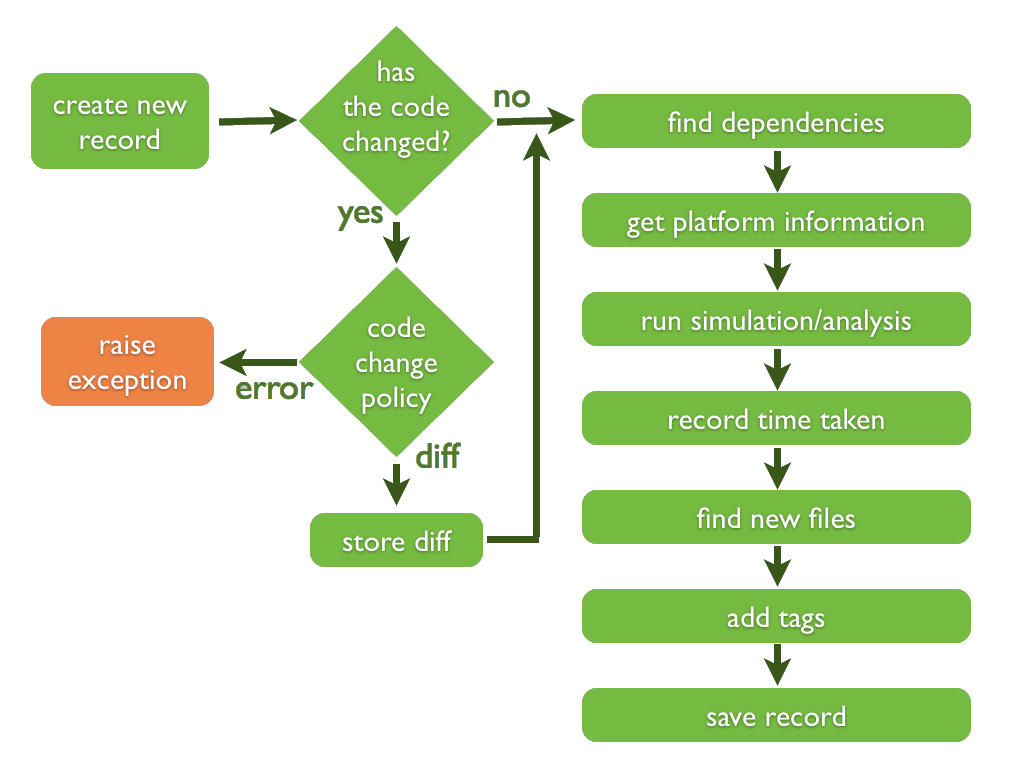
\includegraphics[width=\textwidth]{%
  img/sumatra_record_flowchart.png} %
\end{figure}


                    
        \end{column}
              %
        \begin{column}{.42\textwidth}
          

          \vspace{-1.2cm}
          
    \begin{center}
      \textit{ {\setstretch{1.2} \Large \enquote{An automated electronic lab notebook for computational research}\\}}
    \end{center}
          
          
          
      
        \end{column}
        %

      \end{columns}
      

    
    
  }

  
  
  %% %\large
  %% \begin{columns}  
  %% %%%%
  %%   \begin{column}{0.34\textwidth}
  %%     \vspace{0.46cm}
  %%     \begin{itemize}[leftmargin=2pt]
  %%       \itemsep18pt
  %%       \item<1->[] Which version of my code did I use?
  %%       \item<2->[] What parameters?
  %%       \item<3->[] \enquote{Why did I do that?}
  %%       \item<4->[] \enquote{It worked yesterday.}
  %%     \end{itemize}
  %%     \vspace{3cm}
  %%   \end{column}
  %%   %%%% 
  %%   \begin{column}{0.65\textwidth}
  %%     %\vspace{-1.35cm}
  %%     \only<1-4>{
  %%       \vspace{0.4cm}

  %%       \begin{figure}
  %%         \centering        
  %%         \includegraphics[width=\textwidth]{%
  %%           phd_filenames.png}
  %%         \vspace{-0.28cm}
  %%         \captionsetup{justification=centering}
  %%         \caption*{%
  %%           \tiny \enquote{Piled Higher and Deeper} by Jorge Cham\\
  %%           \href{www.phdcomics.com}{www.phdcomics.com}}
  %%       \end{figure}
  %%     }

  %%     \only<6->{
  %%       \vspace{0.01cm}
  %%       \begin{center}
  %%         \textbf{\textit{laboratory notebook}}
  %%       \end{center}
  %%       \vspace{-1.25cm}
        
  %%       \begin{figure}
  %%         \centering        
  %%         \includegraphics{victor_horsely.jpg}
  %%         % http://wellcomeimages.org/indexplus/image/M0016267.html
  %%         \vspace{-0.28cm}
  %%         \caption*{%
  %%           \tiny \textcopyright Wellcome Library, London 
  %%           \href{http://creativecommons.org/licenses/by/4.0/}{%
  %%             CC BY 4.0}}
  %%       \end{figure}}
      

  %%     \onslide<7->
  %%     \vspace{-0.72cm}
  %%     \begin{center}
  %%       \textit{... in traditional, experiment-based research}.
  %%     \end{center}
  %%   \end{column}
  %%   %%%%
  %% \end{columns}

\end{frame}

